\documentclass[letterpaper,twocolumn,openany,nodeprecatedcode]{dndbook}

% Use babel or polyglossia to automatically redefine macros for terms
% Armor Class, Level, etc...
% Default output is in English; captions are located in lib/dndstrings.sty.
% If no captions exist for a language, English will be used.
%1. To load a language with babel:
%	\usepackage[<lang>]{babel}
%2. To load a language with polyglossia:
%	\usepackage{polyglossia}
%	\setdefaultlanguage{<lang>}
\usepackage[english]{babel}
%\usepackage[italian]{babel}
% For further options (multilanguage documents, hypenations, language environments...)
% please refer to babel/polyglossia's documentation.

\usepackage[utf8]{inputenc}
\usepackage[singlelinecheck=false]{caption}
\usepackage{lipsum}
\usepackage{listings}
\usepackage{shortvrb}
\usepackage{stfloats}

\captionsetup[table]{labelformat=empty,font={sf,sc,bf,},skip=0pt}

\MakeShortVerb{|}

\lstset{%
  basicstyle=\ttfamily,
  language=[LaTeX]{TeX},
  breaklines=true,
}

\title{The Edge of Oblivion \\
\large Aftermath of a lost world}
\author{Ian Wakely}
\date{\today}

\begin{document}

\frontmatter

\maketitle

\tableofcontents

\mainmatter%

\part{World}

\section{The Old Ones}

- The dragonborn nation/society/whatever is called Kaldalis.

\section{In the Night's Sky}

- The meteors threw tons of dust into the atmostsphere, causing the event known as "The Long Night"
- Meteors happened about 300 years ago
- For a handful of years, not anyone can really tell for sure, the world was mostly dark overcast clouds

\section{From the Ashes}

- The mages that later formed Solaris, figured out how to disperse the dust in the atmostsphere
- The end of The Long Night is known as The Dawning, and is often observed as a blessing from Pelor.

\chapter{Name of coast}

\begin{figure}[h!]
  \centering
  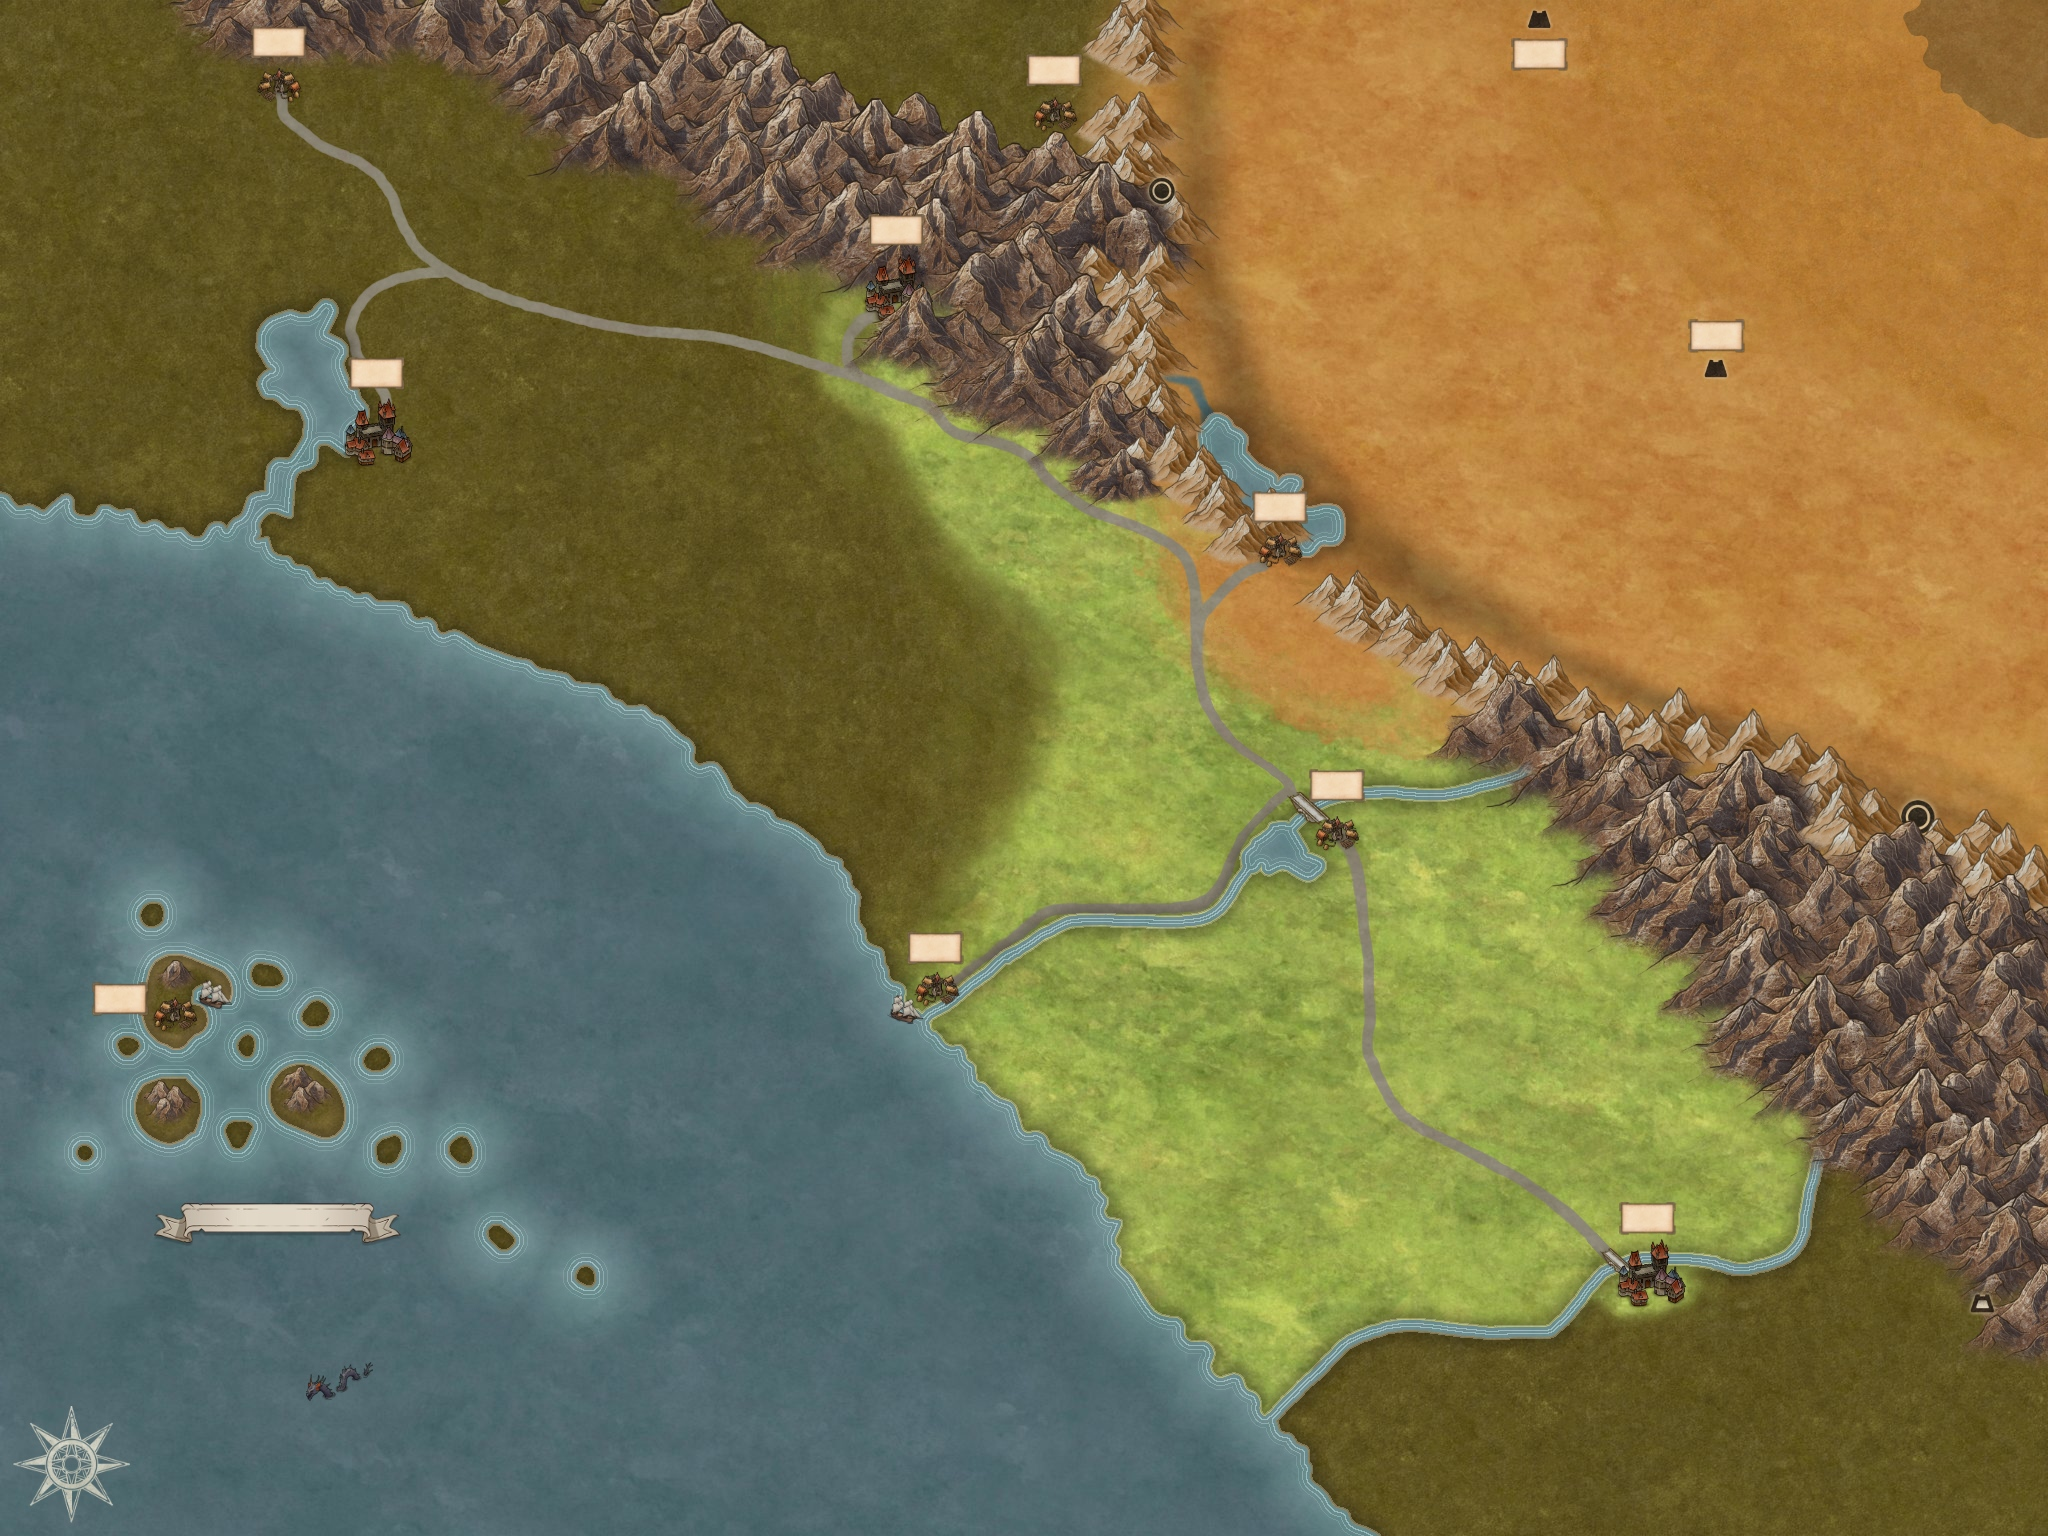
\includegraphics[width=0.45\textwidth]{maps/coastline.jpg}
  \caption{Todo: Figure out how to make this fill width}
\end{figure}

\section{Bastions of Society}

todo

\DndArea{Underthal}

North West mountain village of dwarves in the mountain side. todo: fill in more.

\paragraph{Origin}
todo

\DndArea{Solaris}

A tall city skyline filled with slender towers forming the pinicle of high society of
mages and magic. The city of Solaris is primarily comprised of mages and practitioners
of magic, both of the arcane and of the divine. Governed a councel of eight mages, one
for each of school of magic and masters of their craft, as well as three emissaries of
the major faiths throughout the city.

Solaris is not only the center of magic in this region of the world, but also is the
center of teaching magic in this region of the world. Students from all parts of the
world come to study here.

Seen as a blessing from the Dawn Father, Pelor, the city has a sizeable following of
Pelor, but is just one of many groups of followers within the city.

\paragraph{Origin}
Formed after the dispersion of The Long Night, the newly found brotherhood of mages banded
together to make a new town, later growing into a small city of magic and knowledge.

\DndArea{Harmony}

Previously large Dwarven mine and stronghold of Nulbaraz, now holds a bustling underground
city of Dwarves and Elves in a perfect harmony, which the city now takes as a name in common:
Harmony. Now, the city is governed by a councel of Dwarven and Elven nobals of a city under
the mountain. Mining rare minerals and forging them into all types of good and ofering them
to the world. The city is the epicenter of wealthy merchants of all kinds of mundain items.

\paragraph{Origin}
A number of Elven nobals, using powerful magics, were able to get an early notice of the
impending doom of the world, and begged for the mercy of the Dwarves. With much trepidation,
they allowed the entry of a number of Elven nobals and their families, saving them from their
destruction. They now call their new home after their old one, Anenfel, even though most
others just refer to as Harmony.

\DndArea{Vinyamar}

North middle town. todo: fill in more.

\DndArea{Oblivion}

Found on the edge of the wasteland, Oblivion is not a place for the weak of heart or body.
Mostly made of the rough-and-tumbled type, the dust bowl of a town is made up of adventurers
and explorers either on their way to the wasteland, or on their way to sell something they
stole from someone else.

\paragraph{Origin}
What was first little more that just a wide stop in the road, slowly became a shanty town
of broken people and the broken things they found in the wastes. Trading all kind of mysterious
and misunderstood salvage from the Kaldalis.

\DndArea{Ryefield}

Ryefield has always been an important landmark in the world after the Long Night. It has been a
well needed stop between Knowhere, Oblivion, and the port of Aquarin.  Primarily comprised of
Gnomes and Halflings, the hearty and jovial people enjoy a great time drinking and lauphing
into all hours of the night. For one of the largest towns on the coast, it's center is
relatively small for most of the town's residence live closer to the fields they that take
care of, frequenting the town properly for trade and processing of their fresh crop in one
of the remaining Faro processing facilities.

\paragraph{Origin}
The town was once an automated farm for the Faro corperation. After the destruction of the
of the world, most of the workers and died in the Long Night that followed, the rest stuck
by the decrepit facility, still trying to make the food they needed to survive. The Dawning
brought a bright future to the world, and especially to the town now that it could produce
more food for the people who lived there. Eventually, they grew large enough to produce all
different kinds of things, and trade them with nearby settlements.

\DndArea{Aquarin}
- Sailing town
- Fisherman
- Trade via ship with other distant surviving groups

\paragraph{Origin}
todo

\DndArea{Knowhere}
- Largest City by both size and population
- Previously a large metroplis before the destruction of life
- Heavily over grown with plant life and reclaimed by the land
- Population is a mix of all types of races
- Mostly an industrial city with tons of blacksmiths and artificers

\paragraph{Origin}
todo

\DndArea{Zeffari}
- Small Orc and Lizard folk village
- Want to be left alone
- Deeply religious
- Honor based society
- Live mostly on fish
- Some unknown concret structures
- On the island of Skira

\paragraph{Origin}
todo

\section{The Wastes}

The impact crator left behind by a meteor, was once the center of the powerful Dragonborn
nation, is now a decilate wasteland. Filled with the remains and mysterious of the long
lost empire. The impact threw mountain side and landscape aside, reshaping the land
and destroying a portion of the mountain range.

\DndArea{Ruined City of Xerxes}
todo: Ruins of a larger dagonborn city, Very Dangerous

\DndArea{Ashbourne's Folly}

Wilred Ashbourne, a once skilled adventured, discovered the mostly buried ruins of an
underground Dragonborn facility a number of years ago while exploring The Wastes. After
stumbling upon it, they returned to Oblivion to gather a group to explore the tomb,
and they were never seen or heard from again.

\DndArea{Bunker 4B}

In a shallowy out cropping in the mountains with a large sealed door that has stumped
teasure hunters for a number of years. All that is known about the entrance is that it
was built by the Dragonborn and that there is a large "4B" painted on the door.

\DndArea{TBD}
todo

\section{Starfield Islands}
todo

\section{Organizations}
todo

\subsection{The Trust}
todo

\chapter{Divinity}

\begin{DndTable}{XXXX}
  Deity & Alignment & Province & Suggested Domains \\
  Avandra & CG & Change, freedom, luck & Nature, Trickery \\
  Bahamut & LG & Honor, justice & Life, Order War \\
  Corellon & CG & Art, beauty, elves & Arcana Light \\
  Erathis & LN & Civilization, law, peace & Knowledge, Order \\
  Ioun & N & nowledge, learning, teaching & Arcana Knowledge \\
  Melora & N & Seas, wilderness & Life, Nature, Tempest \\
  Moradin & LG & Craft, creation & Forge Knowledge, War \\
  Pelor & NG & Healing, sun & Life, Light, Nature \\
  Raei & NG & Atonement, compassion & Life, Light \\
  The Raven Queen & LN & Death, fate, winter & Death, Grave \\
  Sehanine & CG & Illusion, moonlight, night & Arcana Nature, Trickery
\end{DndTable}

\section{Old Gods}

Severial of the divine beings and their beliefs were discovered and brought back after the
fall of society, many of whom thought that bringing the faith of The Old Ones back would
help bring back society faster.

\subsection{Bahamut, the Platnum Dragon}

The pillar of justice, protection, nobility, and honor, Bahamut is a beacon to
paladins of order and good, and is revered by most metallic dragons as the first of
their kind. The crest of the Platinum Dragon adorns many halls of high leadership and
justice, invoking his will in all matters of justice. To follow him is to look after
those who cannot look after themselves.

When not wandering the Outer Planes, Bahamut resides within his magnificent, glittering
palace of gold, platinum, and mithril hidden among the winds of the Seven Heavens of Celestia.

\subparagraph{Depiction}
The Platinum Dragon is often seen emblazoned on shields and armor, both functional and
decorative, in the form of a brilliant dragon head in profile. Temples and works of art
depict a massive, glittering dragon with vibrant platinum scales and seemingly
endless wingspan.

\subparagraph{Common Symbol}
Silver dragon’s head in profile.

\subsection{Corellon, the Arch Heart}

Guardian of spring, beauty, and the arts, Corellon is the patron of arcane magic and
the fey. The Founding inspired them to wander the twisted lands, seeding them with the
first arcane magics and raising the most ancient of forests. It was by the Arch Heart’s
hand that the first elves wandered from the Feywild, and for this reason they are
considered the Mother and Father of all elves. Those who seek art in all their work,
whether magical or mundane, often worship at the altar of Corellon. They loathe the
Spider Queen and her priestesses for leading the drow astray.

Corellon watches the business of mortals and gods from within the palace of Crescent
Grove in the beautiful realm of Arborea, surrounded by towering white trees and
pillars of marble.

\subparagraph{Depiction}
Most modern tapestries and tomes depict the Arch Heart as an elven being of impossible
grace and beauty, androgynous and alluring, framed by long, wavy, golden hair. They were
the inspiration for many early elven art pieces, and elements of their visage or symbol
are included in most elven architecture.

\subparagraph{Common Symbol}
Two crescent moons facing each other atop a four-pointed star.

\subsection{Erathis, the Law Bearer}

The inspiration behind many great inventions, the creation of vast cities, and law and
order within society, Erathis claims dominion over civilization. Judges and rulers pay
respect at her temples, which are central structures in many cities across Exandria.
Peace and order through structure and law guides the will of her devout followers.
The Law Bearer has a tempestuous romance with Melora the Wild Mother, a furious love
that is tempered only when civilization and nature are in balance.

Erathis resides within the glorious divine metropolis of Hestavar, the Bright City.
This glowing oasis coasts through the Astral Plane, as the Law Bearer watches over the
denizens bathed in the endless daytime that illuminates the busy streets.

\subparagraph{Depiction}
Erathis is shown in most texts and statues as a hooded, armored woman sitting atop a
throne of pillars. Her face is generally obscured or depicted without expression,
giving her presence an impartial yet imposing nature.

\subparagraph{Common Symbol}
Double-headed axe inset with a pattern of scales

\subsection{Moradin, the All-Hammer}

Moradin is worshiped by smiths, artisans, and miners alike, granting inspiration in
exchange for respect and prayer. He shaped the mountains from the chaos of the Founding,
and stands as the patron protector of home and family. The devotion to the All-Hammer is
strongest in dwarven communities, and many temples to Moradin mark the center of a mighty
dwarven stronghold.

Moradin lords over the soul forges within the massive tunneled mansion of Erackinor,
deep beneath the slopes of Solania on the plane of Celestia.

\subparagraph{Depiction}
Many guild halls and workshops contain images of Moradin, a faceless, stout dwarven
being of immense strength, hunched over a flaming heart clasped within his massive hands.

\subparagraph{Common Symbol}
Hammer with ends carved in the likeness of dwarven heads.

\subsection{The Raven Queen, Matron of Death}

Master of the skein of fate and the mistress of winter, the Raven Queen is the god of
death. Her gaze follows and marks the end of each mortal life, watching over the border
between life and death and ensuring the natural transition is undefiled. Many funerals
ask her blessing to protect the deceased from the terrible curse of undeath. Those who
study ancient lore believe that the Matron of Death was once mortal herself and is the
only known mortal to have ascended to godhood. Her rise instantly obliterated the previous,
now-forgotten god of death, and the other gods quickly and fearfully destroyed the secrets
to the rites of ascension.

The Raven Queen tugs at the threads of fate from her stronghold of black ice within the
frozen realm of Letherna, nestled in a frigid corner of the Shadowfell.

\subparagraph{Depiction}
Few existing visual depictions of the Raven Queen exist; many temples merely use the
raven as a symbol of her blessing. The few illustrations of her portray a tall, pale
woman wrapped in dangling black linens, with her face obscured by a white porcelain
mask and her onyx-black hair straight and neverending.

\subparagraph{Common Symbol}
White, humanoid mask framed in black feathers.

\section{New Gods}

As the world started to reborn from the ashes of The Olds Ones, they started to hope and
pray in new things and ideals. Thanksful for this second chance they were blessed with,
and hoping to do great things with the blessing they received, and hoping to not make
the same "mistakes" that The Old Ones made that caused their downfall.

\subsection{Avanda, the Change Bringer}

Also known as "She Who Makes the Path," Avandra champions freedom, travel, trade, and
adventure across the lands. Her will heralds open frontiers, and her call beckons her
followers to discover that which awaits them beyond the known. There are few urban temples
dedicated to the Change Bringer, but her shrines are often found along well-traveled roads
and off the beaten path. Her worship is common among merchants, free spirits, and adventurers,
and tavern cheers celebrate her as a bringer of luck and fortune.

Avandra calls no domain in the planes her residence, instead eternally wandering through the
Outer Planes where serenity can be found, distantly watching over the potential of mortals.

\subparagraph{Depiction}
The Change Bringer is often depicted as a young woman of dark complexion and long, light brown
hair that cascades to form the road left behind her. Most art shows her in constant motion,
ever leading into the unknown.

\subparagraph{Common Symbol}
Woman’s profile embossed on a gold coin or pendant.

\subsection{Ioun, the Knowing Mentor}

Revered by seers, sages, and teachers of all walks of life, Ioun guided the growth of
civilization throughout the Age of Arcanum like sunlight guides the branches of a tree.
Grievously wounded by the Chained Oblivion during the Calamity, her followers are now
hunted by agents of her ancient foes as she recovers. Her devout now worship in private,
spreading knowledge, philosophy, and lore anonymously through traceless channels.

Ioun sits among the infinite library that fills the hidden realm of the Endless Athenaeum,
her celestial servants cataloging all known things as she inspires those who pray for
her insight and guidance.

\subparagraph{Depiction}
Common representations show the Knowing Mentor as a graying, mature woman with a welcoming,
matronly smile, swathed in billowing robes and scarves that fan into books and scrolls.
Some colloquially refer to Ioun as the Knowing Mistress, revering her as a headmistress
of knowledge among the gods.

\subparagraph{Common Symbol}
Pair of open eyes crowned with a third open eye.

\subsection{Melora, the Wild Mother}

The realm of Melora extends to wherever the seas shift and the land grows wild. As the
keeper of the wilderness, Melora represents the wild creatures of nature, the rush of the
angry rapids, and the heat-heavy stillness of the desert. Elves worship her, as do hunters,
accepting her guidance to exist harmoniously within savage lands. Those seeking safe passage
across dangerous waters pray to her to guide them.

Followers of the Raven Queen also show respect to the Wild Mother as the caretaker of
what remains when the Matron of Death’s work is done. Those of Ki’Nau descent often make
offerings to Melora, considering her a collective entity that represents their ancient nature
gods within a singular feminine form. Druids of Melora the Wild Mother and clerics of her
lover, Erathis the Law Bearer, work together to preserve the balance of nature and
civilization. However, worship of Melora was outlawed in the Dwendalian Empire, causing
disagreement between clerics of Erathis within Western Wynandir, where many blame poor
weather and natural disasters on the ire of their deity’s partner.

Eschewing a permanent realm, Melora prefers to wander the planes to oversee natural life.
She is often found among the unearthly beauty of Arvandor’s infinite expanse of deep woods,
hunting unnatural things that corrupt the wilds.

\subparagraph{Depiction}
Immortalized through wooden reliefs and carved idols in hidden, overgrown groves and rural
shrines, the Wild Mother is shown as a beautiful woman with green skin nearly swallowed by
a wild, tangled wreath of hair, leaves, and vines that dwarf her lithe form.

\subparagraph{Common Symbol}
Wreath of grass and grain affixed to a crook.

\subsection{Pelor, the Dawn Father}

Pelor rules over sun and summer, his vigil encircling the ages as the keeper of time. As
lord of agriculture and harbinger of the harvest, he is worshiped by farmers and most common
folk, and his priests are welcomed in many lands. Supporter of the needy and destroyer of
evil, the Dawn Father is often the patron of paladins and rangers who follow a similar creed.
He is also known for his defeat of the Chained Oblivion and is revered by those who
hunt aberrations.

Pelor is often found within the Fortress of the Sun, a shining, golden citadel that brings
vibrant life to the limitless orchards of the Blessed Fields of Elysium.

\subparagraph{Decpition}
Tapestries of old match early texts describing Pelor as a paternal figure in silver and
gold armor, his head a beacon of light and fire so bright that his face can barely be seen.
Many statues in holy places use the head as a brazier, lit with each dawn and extinguished
at dusk.

\subparagraph{Common Symbol}
Bright, eight-pointed star.

\subsection{Raei, the Everlight}

God of atonement and compassion, Raei spreads the message of understanding and optimism in
even the darkest of places. She believes that the corrupt can be redeemed, a mindset that led
to a betrayal by the Lord of the Nine Hells, who decimated her followers during the Calamity.
This misplaced trust caused many priests to strike her name from historical records, leaving
her title and faith scattered to obscurity for much of the recent age. Only recently has her
faith been rediscovered and her temples returned to prominence. The Everlight’s followers are
often rural healers and community philosophers, offering a voice of reason and empathy in
angry and cynical times.

Raei guides her people from within her temple beside the crystal beaches of the Island of
Renewal, a hidden sanctuary of flame alongside the Blessed Fields of Elysium.

\subparagraph{Depiction}
Those who bring the Everlight’s words back to the light unearth her image from ruined temples,
or create new art to inspire others with her message. Raei is represented as a beautiful,
strong woman with dark skin and light hair, rising betwixt a set of angelic ivory wings.

\subparagraph{Common Symbol}
Humanoid, feminine phoenix.

\subsection{Sehanine, the Moon Weaver}

Sehanine is the god of moonlight and the autumn season, as well as the patron of illusions
and misdirection. Widely worshiped in halfling and elven cultures, she is considered to be
the deity of love, protecting the trysts of lovers with shadows of her own making. Those who
work in darkness and trickery often ask for her blessing.

Sehanine is found among the verdant tangles of the realm of Arborea, watching over the elven
courts, or wandering among the colorful fields of the Feywild.

\subparagraph{Depiction}
The Moon Weaver’s depictions are as numerous as the myths and stories of her meddling with
the unions of mortals. She is most often painted as a young girl with light-blue skin and
white hair, her body and limbs merely wavy silk strands of silver moonlight that caress and
create the edges of the shadows around her.

\subparagraph{Common Symbol}
Crescent moon turned upward, strung like a bow.

\part{Layout Notes}

\chapter{Sections}

\DndDropCapLine{T}{his package is designed to aid you in} writing beautifully typeset documents for the fifth edition of the world's greatest roleplaying game. It starts by adjusting the section formatting from the defaults in \LaTeX{} to something a bit more familiar to the reader. The chapter formatting is displayed above.

\section{Section}
Sections break up chapters into large groups of associated text.

\subsection{Subsection}
Subsections further break down the information for the reader.

\subsubsection{Subsubsection}
Subsubsections are the furthest division of text that still have a block header. Below this level, headers are displayed inline.

\paragraph{Paragraph}
The paragraph format is seldom used in the core books, but is available if you prefer it to the ``normal'' style.

\subparagraph{Subparagraph}
The subparagraph format with the paragraph indent is likely going to be more familiar to the reader.

\section{Special Sections}
The module also includes functions to aid in the proper typesetting of multi-line section headers: |\DndFeatHeader| for feats, |\DndItemHeader| magic items and traps, and |\DndSpellHeader| for spells.

\DndFeatHeader{Typesetting Savant}[Prerequisite: \LaTeX{} distribution]
You have acquired a package which aids in typesetting source material for one of your favorite games, giving you the following benefits:

\begin{itemize}
  \item You have advantage on Intelligence checks to typeset new content.
  \item When you fail an Intelligence check to typeset new content, you can ask questions online at the package's website.
\end{itemize}

\DndItemHeader{Foo's Quill}{Wondrous item, rare}
This quill has 3 charges. While holding it, you can use an action to expend 1 of its charges. The quill leaps from your hand and writes a contract applicable to your situation.

The quill regains 1d3 expended charges daily at dawn.

\DndSpellHeader%
  {Beautiful Typesetting}
  {4th-level illusion}
  {1 action}
  {5 feet}
  {S, M (ink and parchment, which the spell consumes)}
  {Until dispelled}
You are able to transform a written message of any length into a beautiful scroll. All creatures within range that can see the scroll must make a wisdom saving throw or be charmed by you until the spell ends.

While the creature is charmed by you, they cannot take their eyes off the scroll and cannot willingly move away from the scroll. Also, the targets can make a wisdom saving throw at the end of each of their turns. On a success, they are no longer charmed.

\section{Map Regions}
The map region functions |\DndArea| and |\DndSubArea| provide automatic numbering of areas.

\DndArea{Village of Hommlet}
This is the village of hommlet.

\DndSubArea{Inn of the Welcome Wench}
Inside the village is the inn of the Welcome Wench.

\DndSubArea{Blacksmith's Forge}
There's a blacksmith in town, too.

\DndArea{Foo's Castle}
This is foo's home, a hovel of mud and sticks.

\DndSubArea{Moat}
This ditch has a board spanning it.

\DndSubArea{Entrance}
A five-foot hole reveals the dirt floor illuminated by a hole in the roof.

\chapter{Text Boxes}

The module has three environments for setting text apart so that it is drawn to the reader's attention. |DndReadAloud| is used for text that a game master would read aloud.

\begin{DndReadAloud}
  As you approach this module you get a sense that the blood and tears of many generations went into its making. A warm feeling welcomes you as you type your first words.
\end{DndReadAloud}

\section{As an Aside}
The other two environments are the |DndComment| and the |DndSidebar|. The |DndComment| is breakable and can safely be used inline in the text.

\begin{DndComment}{This Is a Comment Box!}
  A |DndComment| is a box for minimal highlighting of text. It lacks the ornamentation of |DndSidebar|, but it can handle being broken over a column.
\end{DndComment}

The |DndSidebar| is not breakable and is best used floated toward a page corner as it is below.

\begin{DndSidebar}[float=!b]{Behold the DndSidebar!}
  The |DndSidebar| is used as a sidebar. It does not break over columns and is best used with a figure environment to float it to one corner of the page where the surrounding text can then flow around it.
\end{DndSidebar}

\section{Tables}
The |DndTable| colors the even rows and is set to the width of a line by default.

\begin{DndTable}[header=Nice Table]{XX}
    Table head  & Table head \\
    Some value  & Some value \\
    Some value  & Some value \\
    Some value  & Some value
\end{DndTable}

\chapter{Monsters and NPCs}

% Monster stat block
\begin{DndMonster}[float*=b,width=\textwidth + 8pt]{Monster Foo}
  \begin{multicols}{2}
    \DndMonsterType{Medium aberration (metasyntactic variable), neutral evil}

    % If you want to use commas in the key values, enclose the values in braces.
    \DndMonsterBasics[
        armor-class = {9 (12 with \emph{mage armor})},
        hit-points  = {\DndDice{3d8 + 3}},
        speed       = {30 ft., fly 30 ft.},
      ]

    \DndMonsterAbilityScores[
        str = 12,
        dex = 8,
        con = 13,
        int = 10,
        wis = 14,
        cha = 15,
      ]

    \DndMonsterDetails[
        %saving-throws = {Str +0, Dex +0, Con +0, Int +0, Wis +0, Cha +0},
        %skills = {Acrobatics +0, Animal Handling +0, Arcana +0, Athletics +0, Deception +0, History +0, Insight +0, Intimidation +0, Investigation +0, Medicine +0, Nature +0, Perception +0, Performance +0, Persuasion +0, Religion +0, Sleight of Hand +0, Stealth +0, Survival +0},
        %damage-vulnerabilities = {cold},
        %damage-resistances = {bludgeoning, piercing, and slashing from nonmagical attacks},
        %damage-immunities = {poison},
        %condition-immunities = {poisoned},
        senses = {darkvision 60 ft., passive Perception 10},
        languages = {Common, Goblin, Undercommon},
        challenge = 1,
      ]
    % Traits
    \DndMonsterAction{Innate Spellcasting}
    Foo's spellcasting ability is Charisma (spell save DC 12, +4 to hit with spell attacks). It can innately cast the following spells, requiring no material components:
    \begin{DndMonsterSpells}
      \DndInnateSpellLevel{misty step}
      \DndInnateSpellLevel[3]{fog cloud, rope trick}
      \DndInnateSpellLevel[1]{identify}
    \end{DndMonsterSpells}

    \DndMonsterAction{Spellcasting}
    Foo is a 2nd-level spellcaster. Its spellcasting ability is Charisma (spell save DC 12, +4 to hit with spell attacks). It has the following sorcerer spells prepared:
    \begin{DndMonsterSpells}
      \DndMonsterSpellLevel{blade ward, fire bolt, light, shocking grasp}
      \DndMonsterSpellLevel[1][3]{burning hands, mage armor, shield}
    \end{DndMonsterSpells}

    \DndMonsterSection{Actions}
    \DndMonsterAction{Multiattack}
    The foo makes two melee attacks.

    %Default values are shown commented out
    \DndMonsterAttack[
      name=Dagger,
      %distance=both, % valid options are in the set {both,melee,ranged},
      %type=weapon, %valid options are in the set {weapon,spell}
      mod=+3,
      %reach=5,
      %range=20/60,
      %targets=one target,
      dmg=\DndDice{1d4+1},
      dmg-type=piercing,
      %plus-dmg=,
      %plus-dmg-type=,
      %or-dmg=,
      %or-dmg-when=,
      %extra=,
    ]

    %\DndMonsterMelee calls \DndMonsterAttack with the melee option
    \DndMonsterMelee[
      name=Flame Tongue Longsword,
      mod=+3,
      %reach=5,
      %targets=one target,
      dmg=\DndDice{1d8+1},
      dmg-type=slashing,
      plus-dmg=\DndDice{2d6},
      plus-dmg-type=fire,
      or-dmg=\DndDice{1d10+1},
      or-dmg-when=if used with two hands,
      %extra=,
    ]

    %\DndMonsterRanged calls \DndMonsterAttack with the ranged option
    \DndMonsterRanged[
      name=Assassin's Light Crossbow,
      mod=+1,
      range=80/320,
      dmg=\DndDice{1d8},
      dmg-type=piercing,
      %plus-dmg=,
      %plus-dmg-type=,
      %or-dmg=,
      %or-dmg-when=,
      extra={, and the target must make a DC 15 Constitution saving throw, taking 24 (7d6) poison damage on a failed save, or half as much damage on a successful one}
    ]

    % Legendary Actions
    \DndMonsterSection{Legendary Actions}
    The foo can take 3 legendary actions, choosing from the options below. Only one legendary action option can be used at a time and only at the end of another creature's turn. The foo regains spent legendary actions at the start of its turn.

    \begin{DndMonsterLegendaryActions}
      \DndMonsterLegendaryAction{Move}{The foo moves up to its speed.}
      \DndMonsterLegendaryAction{Dagger Attack}{The foo makes a dagger attack.}
      \DndMonsterLegendaryAction{Create Contract (Costs 3 Actions)}{The foo presents a contract in a language it knows and waves it in the face of a creature within 10 feet. The creature must make a DC 10 Intelligence saving throw. On a failure, the creature is incapacitated until the start of the foo's next turn. A creature who cannot read the language in which the contract is written has advantage on this saving throw.}
    \end{DndMonsterLegendaryActions}
  \end{multicols}
\end{DndMonster}

The |DndMonster| environment is used to typeset monster and NPC stat blocks. The module supplies many functions to easily typeset the contents of the stat block

\part{Customization}

\chapter{Colors}

\begin{table*}[b]
  \caption{\DndFontTableTitle{}Colors Supported by this Package}\label{tab:colors}

  \begin{tabularx}{\linewidth}{lX}
    \textbf{Color}                  & \textbf{Description} \\
    \rowcolor{PhbLightGreen}
    |PhbLightGreen|                 & Light green used in PHB Part 1 (Default) \\
    \rowcolor{PhbLightCyan}
    |PhbLightCyan|                  & Light cyan used in PHB Part 2 \\
    \rowcolor{PhbMauve}
    |PhbMauve|                      & Pale purple used in PHB Part 3 \\
    \rowcolor{PhbTan}
    |PhbTan|                        & Light brown used in PHB appendix \\
    \rowcolor{DmgLavender}
    |DmgLavender|                   & Pale purple used in DMG Part 1 \\
    \rowcolor{DmgCoral}
    |DmgCoral|                      & Orange-pink used in DMG Part 2 \\
    \rowcolor{DmgSlateGray}
    |DmgSlateGray| (|DmgSlateGrey|) & Blue-gray used in PHB Part 3 \\
    \rowcolor{DmgLilac}
    |DmgLilac|                      & Purple-gray used in DMG appendix \\
    \rowcolor{BrGreen}
    |BrGreen|                       & Gray-green used for tables in Basic Rules\\
  \end{tabularx}
\end{table*}

This package provides several global color variables to style |DndComment|, |DndReadAloud|, |DndSidebar|, and |DndTable| environments.

\begin{DndTable}[header=Box Colors]{lX}
  Color            &  Description \\
  |commentcolor|   & |DndComment| background \\
  |readaloudcolor| & |DndReadAloud| background \\
  |sidebarcolor|   & |DndSidebar| background \\
  |tablecolor|     & background of even |DndTable| rows \\
\end{DndTable}

They also accept an optional color argument to set the color for a single instance. See Table~\ref{tab:colors} for a list of core book accent colors.

\begin{lstlisting}
\begin{DndTable}[color=PhbLightCyan]{cX}
  d8 & Item \\
  1  & Small wooden button \\
  2  & Red feather \\
  3  & Human tooth \\
  4  & Vial of green liquid \\
  6  & Tasty biscuit \\
  7  & Broken axe handle \\
  8  & Tarnished silver locket \\
\end{DndTable}
\end{lstlisting}

\begin{DndTable}[color=PhbLightCyan]{cX}
  d8 & Item \\
  1  & Small wooden button \\
  2  & Red feather \\
  3  & Human tooth \\
  4  & Vial of green liquid \\
  6  & Tasty biscuit \\
  7  & Broken axe handle \\
  8  & Tarnished silver locket \\
\end{DndTable}

\section{Themed Colors}
Use |\DndSetThemeColor[<color>]| to set |commentcolor|, |readaloudcolor|, |sidebarcolor|, and |tablecolor| to a specific color. Calling |\DndSetThemeColor| without an argument sets those colors to the current |themecolor|. In the following example the group limits the change to just a few boxes; after the group finishes, the colors are reverted to what they were before the group started.

\begin{lstlisting}
\begingroup
\DndSetThemeColor[PhbMauve]

\begin{DndComment}{This Comment Is in Mauve}
  This comment is in the the new color.
\end{DndComment}

\begin{DndSidebar}{This Sidebar Is Also Mauve}
  The sidebar is also using the new theme color.
\end{DndSidebar}
\endgroup
\end{lstlisting}

\begingroup
\DndSetThemeColor[PhbMauve]

\begin{DndComment}{This Comment Is in Mauve}
  This comment is in the the new color.
\end{DndComment}

\begin{DndSidebar}{This Sidebar Is Also Mauve}
  The sidebar is also using the new theme color.
\end{DndSidebar}
\endgroup

\end{document}
